\section{Cryptoeconomics}

We now present our economical analysis on \name. We have
already discussed that the NIPoPoW protocol is performed in distinct phases. In
each phase, different entities are prompted to act. As in SPV, the security
assumption that is made is that at least one honest node is connected to the
verifier contract and serves honest proofs. However, the process of contesting
a submitted proof by a honest node does not come without expenses.  Such an
expense is the computational power a node has to consume in order to fetch a
submitted proof from the calldata and construct a contesting proof, but most
importantly, the gas that has to be paid in order to dispatch a the proof to
the Ethereum blockchain. Therefore, it is essential to provide motives to
nodes, while, adversaries have to be dishearten from
submitting invalid proofs.  We refer to the principle of promoting honest
actions against adversarial actions as ``fairness''.

In NIPoPoWs, fairness is addressed by the establishment of a monetary value
termed collateral. In \emph{submit} phase, the user pays this collateral in
addition to the expenses of the function call, and, if the proof is contested
successfully, the collateral is paid to the user that achieves to invalidate
the proof. If the proof is not contested, then the collateral is returned to
the original issuer. This treatment incentivizes nodes to participate to the
protocol, and discourages adversaries from joining. It is critical that the
collateral covers all the expenses of the entity issuing the contest.

\noindent \textbf{Collateral.} The determination of a fair collateral is not
trivial. Thorough analysis has to be made regarding to the gas consumption of
all involved phases, as well as the immediacy of required actions. In the
Ethereum blockchain, the priority of transactions is determined by the gas
price~\cite{wood} a user assigns to the underlying transaction. This means that
the user can chose the estimated time in which transactions are published.
Since the duration of contest period in NIPoPoWs is bounded by a finite number
of rounds $n$, the probability of the contesting proof to be included within the
following $n$ blocks must be significant. Otherwise, it is possible for an invalid
proof to be established due to the lack of challenge. Albeit the user that
initiates the submission may demand a direct interaction, and thus selects a
high gas price, the value of the collateral is not affected, as the burden
of the contester is not determined by the priority of the publication of the initial
proof.

\noindent \textbf{Analysis.} We examine various cases in which an invalid
submission is followed by a successful contest. Generally, we expect for an
adversary to provide a proof of a chain that is a fork of the honest chain at
some index relatively close to the tip. This is due to the fact that the
ability of an adversary to sustain a fork chain is exponentially weakened as
the honest chain progresses. We consider a fork of 100 blocks sufficient to
describe an attempt of a power adversary. However, we examine further cases.
Our experiments include fraud proofs of chains that fork an honest Bitcoin-like
chain $100$, $100{,}000$ and $650{,}000$ blocks prior to the tip. The last
experiment essentially represents the case of selfish mining~\cite{selfish}
from Bitcoin's genesis. We define as $\textsf{Z}$ the profit the node gains in
case of a successful contest so that the collateral equals to \textsf{Z} + the
expended gas. We consider $0.1$ Ether (\$2) to be a sufficient amount for
\textsf{Z}. Note that, different gas prices formulate different costs for
contest.

We use ETH Gas Station~\cite{eth-gas-station} to calculate the probabilities of
transactions' inclusions with respect to gas price, a tool that is widely used
by the Ethereum community. In Figure~\ref{fig:cryptoeconomics}, we illustrate
the economical analysis of our client. Green and blue solid lines in each graph
display the transaction cost in USD for each phase as a function of the gas
price. The red solid line in each graph represents the collateral as a function
of the probability of the contest transaction's inclusion in the following 200
blocks. As this probability approaches 1, the gas price needs to be increased.
Dashed lines illustrate the total cost of a submission in USD for several
selections of collateral, as a product of desired value of gas price. The
selection for gas price of the submit phase does not affect collateral, but
dictates the immediacy of the transaction by the user.

In Figure~\ref{fig:cryptoeconomics-100} we observe that the transaction cost of
a submission for a chain that equals the length of Bitcoin as a mid priority
transaction (80\% probability of getting accepted in the next 200 blocks) is
\$9.25, while the contest transaction in very high priority (100\% probability
of being included in the next 200 blocks) is \$7.99. The collateral in this
case is \$9.99 (contest cost+\textsf{Z}).

\begin{figure}[h]
\begin{subfigure}{0.97\linewidth}
    \begin{center}
        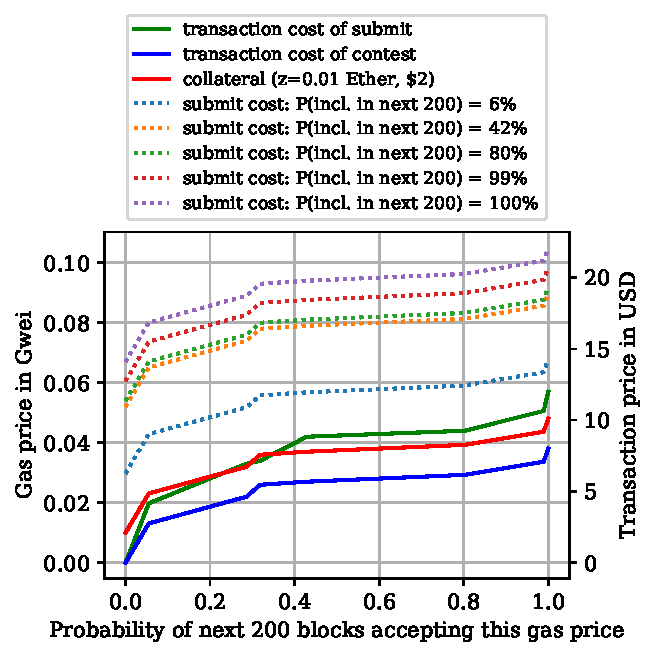
\includegraphics[width=1\columnwidth]{figures/cryptoeconomics-100.pdf}
    \end{center}
    \caption{Collateral analysis for fork proof at index 100.}
    \label{fig:cryptoeconomics-100}
\end{subfigure}

\begin{subfigure}{0.97\linewidth}
    \begin{center}
        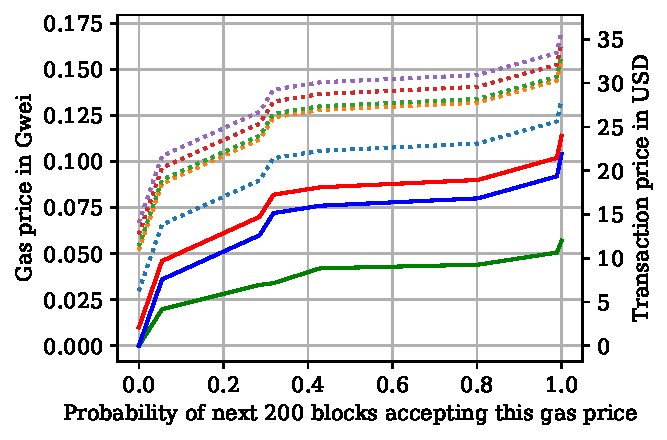
\includegraphics[width=1\columnwidth]{figures/cryptoeconomics-100K.pdf}
    \end{center}
    \caption{Collateral analysis for fork proof at index 100.000.}
    \label{fig:cryptoeconomics-100K}
\end{subfigure}

\begin{subfigure}{0.97\linewidth}
    \begin{center}
        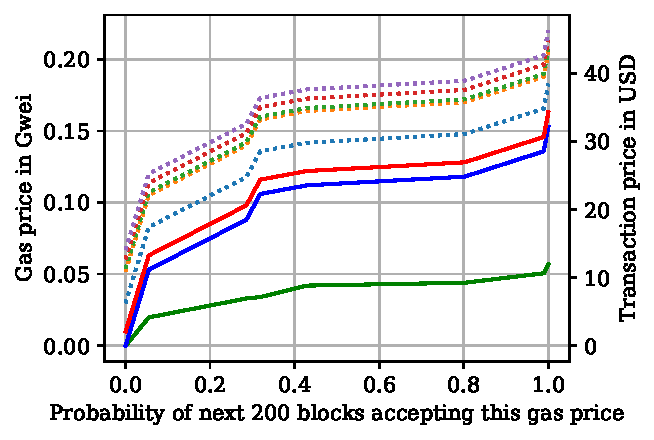
\includegraphics[width=1\columnwidth]{figures/cryptoeconomics-650K.pdf}
    \end{center}
    \caption{Collateral analysis for fork proof at index 650.000.}
    \label{fig:cryptoeconomics-650K}
\end{subfigure}
\caption{Economical analysis of \name.}
\label{fig:cryptoeconomics}
\end{figure}


